\section{Software Reverse Engineering}  
\citep{digitalai_reverse_engineering} states that 
\begin{tcolorbox}[colback=gray!10, colframe=gray!20]
	``The goal of reverse engineering is to reveal the logic, features, and functionalities embedded within the software.''
\end{tcolorbox}

An article by~\citep{twoFacesOfSRE} discusses that software reverse engineering can be achieved through several approaches:
\begin{itemize}
    \item \textbf{Observation-Based Analysis:} Involves studying the exchange of information within the software to infer its functionality and behavior.
    \item \textbf{Disassembly:} Utilizes a disassembler to interpret and analyze the program's raw machine code.
    \item \textbf{Decompilation:} Employs a decompiler to attempt reconstruction of the program’s source code in a high-level language, starting from machine code or bytecode.
\end{itemize}

\begin{figure}[H]
    \centering
    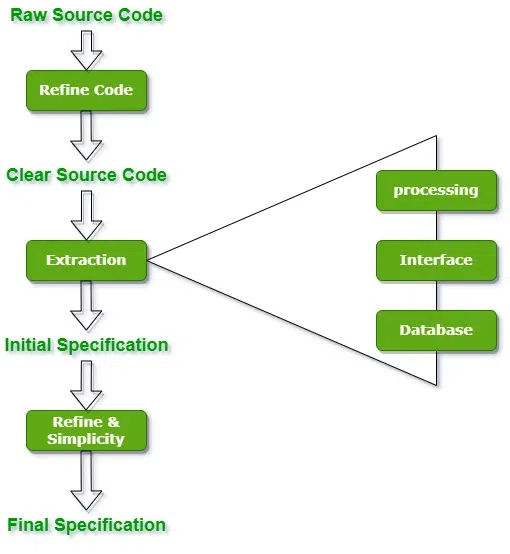
\includegraphics[width=0.75\textwidth]{figures/Reverse-Engineering.png}
    \caption{Reverse Engineering (adapted from~\cite{geeksforgeeks2024})}
	\label{fig_background_reverse_engineering}
\end{figure}

As shown in figure~\ref{fig_background_reverse_engineering}, source code is refined and analyzed to derive a final specification.

\begin{itemize}
    \item The process begins with the raw source code of a software application.
    \item The raw source code is refined to make it cleaner, more organized, and readable by removing unnecessary parts.
    \item The process of extraction identifies key elements of the system.
    \item An initial specification of the system is created, outlining the system's structure and behavior.
    \item The initial specification is then further refined to ensure simplicity and reducing complexity.
    \item The process concludes with a final specification, which is a clear description of the system's design, functionality, and architecture.
\end{itemize}